\documentclass[12pt]{article}
\usepackage{natbib}
\usepackage{hyperref}
\usepackage{graphicx}
\usepackage{caption}
\usepackage{subcaption}

% change document font family to Palatino, and code font to Courier
\usepackage{mathpazo} % add possibly `sc` and `osf` options
\usepackage{eulervm}
\usepackage{courier}

% change page margin
\usepackage[margin=0.8 in]{geometry} 
%title positon
\usepackage{titling} %fix title
\setlength{\droptitle}{-6em}   % Move up the title 

%change section title font size
\usepackage{titlesec} 
\titleformat{\section}
  {\normalfont\fontsize{12}{15}}{\thesection}{1em}{}
\titleformat{\subsection}
  {\normalfont\fontsize{12}{13}}{\thesubsection}{1em}{}
\titleformat{\subsubsection}
  {\normalfont\fontsize{12}{13}}{\thesubsubsection}{1em}{}

%change section title font size


\begin{document}
\title{MIT 6.882 Final Project\\ (Jeremiah) Zhe Liu , Will Townes\\ \today \vspace{-1ex}}

\pretitle{\centering\normalsize}
\posttitle{\par}
\author{}
\date{}
\vspace{-10em}
\maketitle
\vspace{-6em}

\tableofcontents


%\section*{Instructions} %comment out this section before turning in!
% The progress report
% (one  per  team)  will  be  a  written  pdf  document,  about  2  pages  long,
% reporting on what has been accomplished so far and outlining the work that remains to be done.
% You should write clearly about how you've spent your time so far and any preliminary  ndings
% (positive  or  negative).   Then  you  should  include  a  plan  (updated  and/or  revised  from  the  pro-
% posal,  as appropriate) for the time remaining.  If there are multiple participants,  the division of
% responsibility should be made clear.

\newpage
\section{\textbf{Current Progress}}
\subsection{\textbf{Dirichlet Process Sampler}}
We have completed the code for sampling from the DP prior. We have also created the simulated data (Figure \ref{fig:1a}, \ref{fig:1c}, \ref{fig:1d}). We are about half-way through the Gibbs Sampler for sampling from the DP posterior. One obstacle here was we weren't sure whether to use the collapsed sampler (Chinese Restaurant Process) or a blocked sampler. It seems that Fox et al \citep{fox_bayesian_2009} used the latter with a truncated stick-breaking process. Will worked on this part.


\begin{figure*}[h!]
    \centering
    \begin{subfigure}{0.5\textwidth}
        \centering
        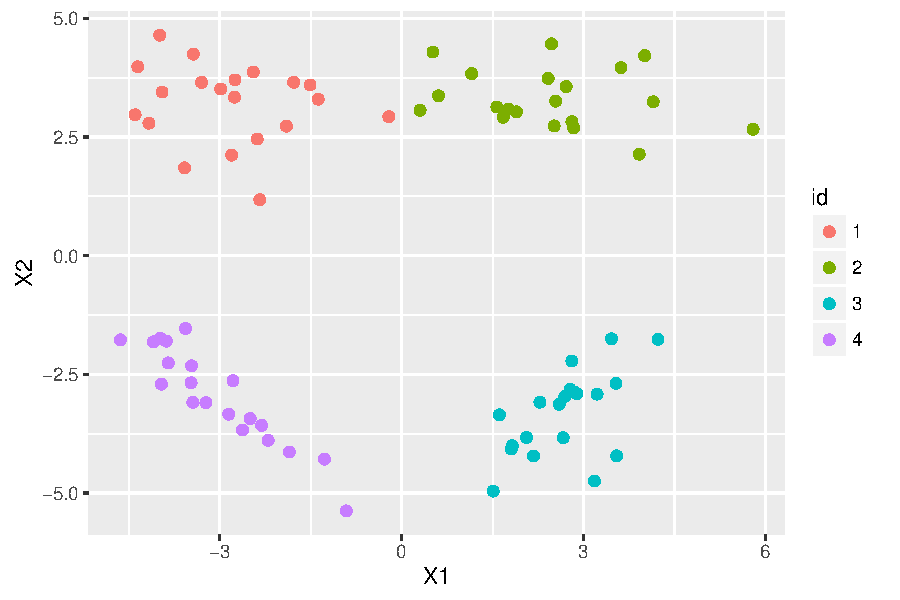
\includegraphics[width = 0.5\linewidth]{plots/gmm.pdf}
        \caption{Test Data for Dirichlet Process Mixture Model: A four-component Gaussian Mixture Model}
        \label{fig:1a}
    \end{subfigure}%
    ~ 
    \begin{subfigure}{0.5\textwidth}
        \centering
        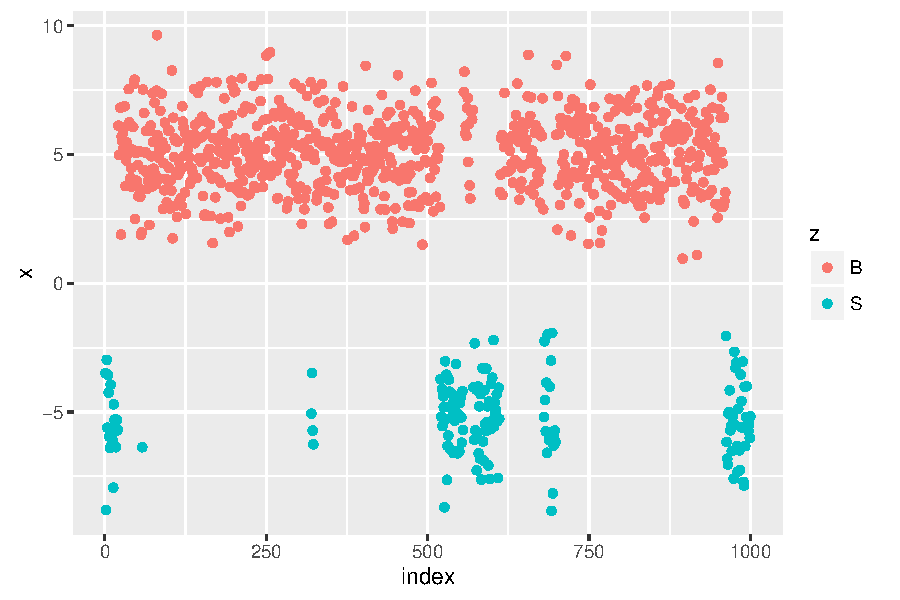
\includegraphics[width = 0.5\linewidth]{plots/hmm.pdf}
        \caption{Test Data for Hidden Markov Model: two hidden states with gaussian emissions}
        \label{fig:1b}        
    \end{subfigure}%
    
    \begin{subfigure}{0.5\textwidth}
        \centering
        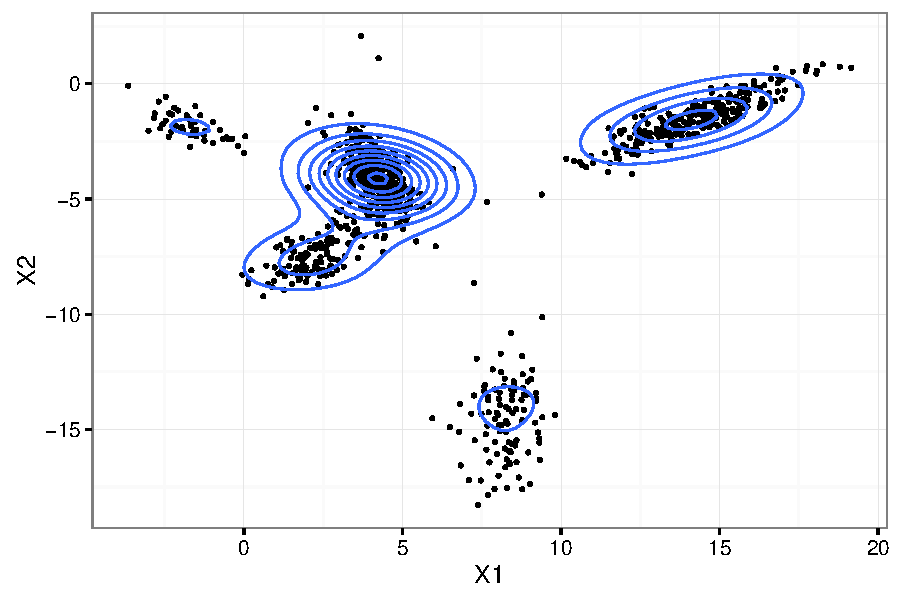
\includegraphics[width = 0.5\linewidth]{plots/DP_GMM1.pdf}
        \caption{Samples from DP mixture of Gaussians Prior}
        \label{fig:1c}
    \end{subfigure}%
    ~
    \begin{subfigure}{0.5\textwidth}
        \centering
        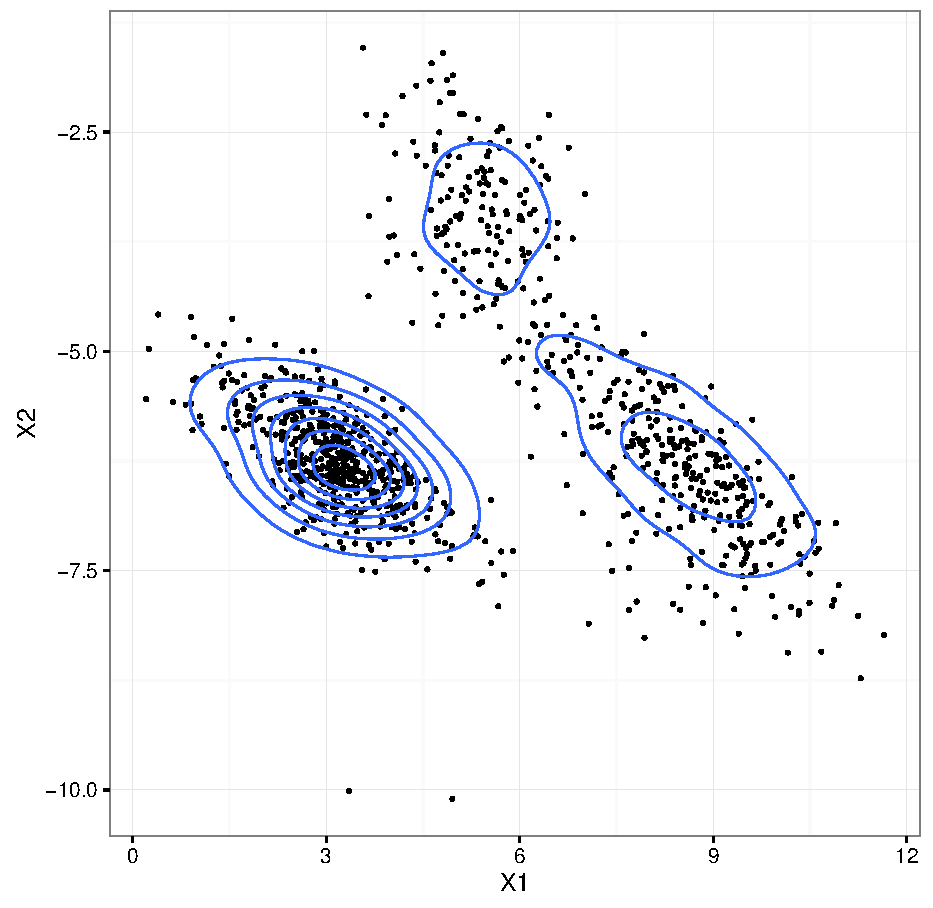
\includegraphics[width = 0.5\linewidth]{plots/DP_GMM2.pdf}
        \caption{Samples from DP mixture of Gaussians Prior}
        \label{fig:1d}
    \end{subfigure}%
    \caption{Test Data/Generated Samples from MDP and HMM models}
 \end{figure*}



\subsection{\textbf{Hierarchical Dirichlet Process Sampler}}
A modularized implementation of HDP sampler (using the direct assignment approach as described in Teh (2006)\citep{teh_hierarchical_2006}) has been completed and available at \href{https://github.com/willtownes/mit6882/tree/jere/jere/func}{GitHub project page}. We have performed preliminary trials on clustered Gaussian data (Figure ) with promising results (Figure ). However, our current implementation suffers some classical problems with DP sampler, such as slow mixing rate for the number of underlying modes, and over-estimation of the number of clusters. We plan to further strengthen our implementation by adding:
\begin{enumerate}
\item Block Sampler: \\
Improve the mixing rate by using a finite-dimensional approximate of DP prior as discussed in Ishwaran and James (2001). \citep{ishwaran_gibbs_2001}
\item Sampling concentration parameters: \\
Since model performance depend largely on the specification of $\gamma$ and $\alpha$, it is advisable to sample the two concentration parameters as well as discussed in Teh (2006) \citep{teh_hierarchical_2006}.
\end{enumerate} 


\begin{figure}
\centering
    \begin{subfigure}{0.5\textwidth}
        \centering
        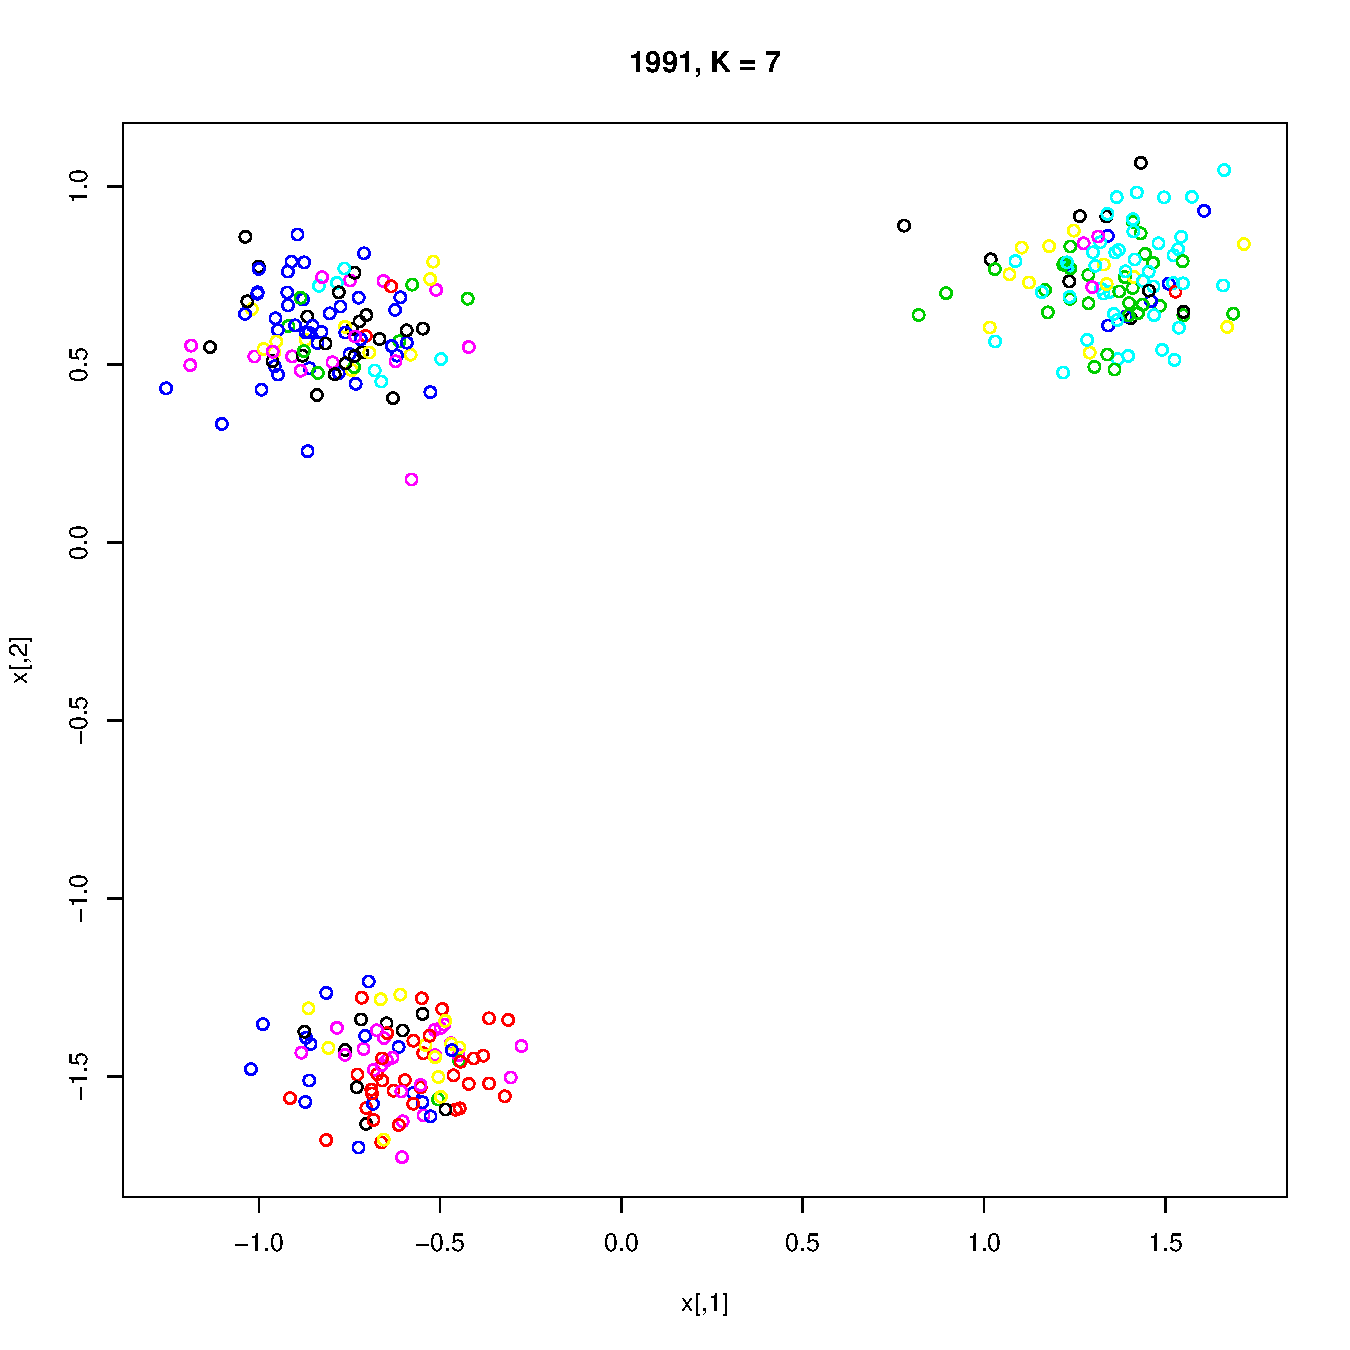
\includegraphics[width = 0.5\linewidth]{plots/hdp_data.pdf}
        \caption{Estimated Cluster Assignment of Gaussian Clustering Data in Iteration 1991/2000, with 7 clusters}
        \label{fig:1d}
    \end{subfigure}%
    ~
    \begin{subfigure}{0.5\textwidth}
        \centering
        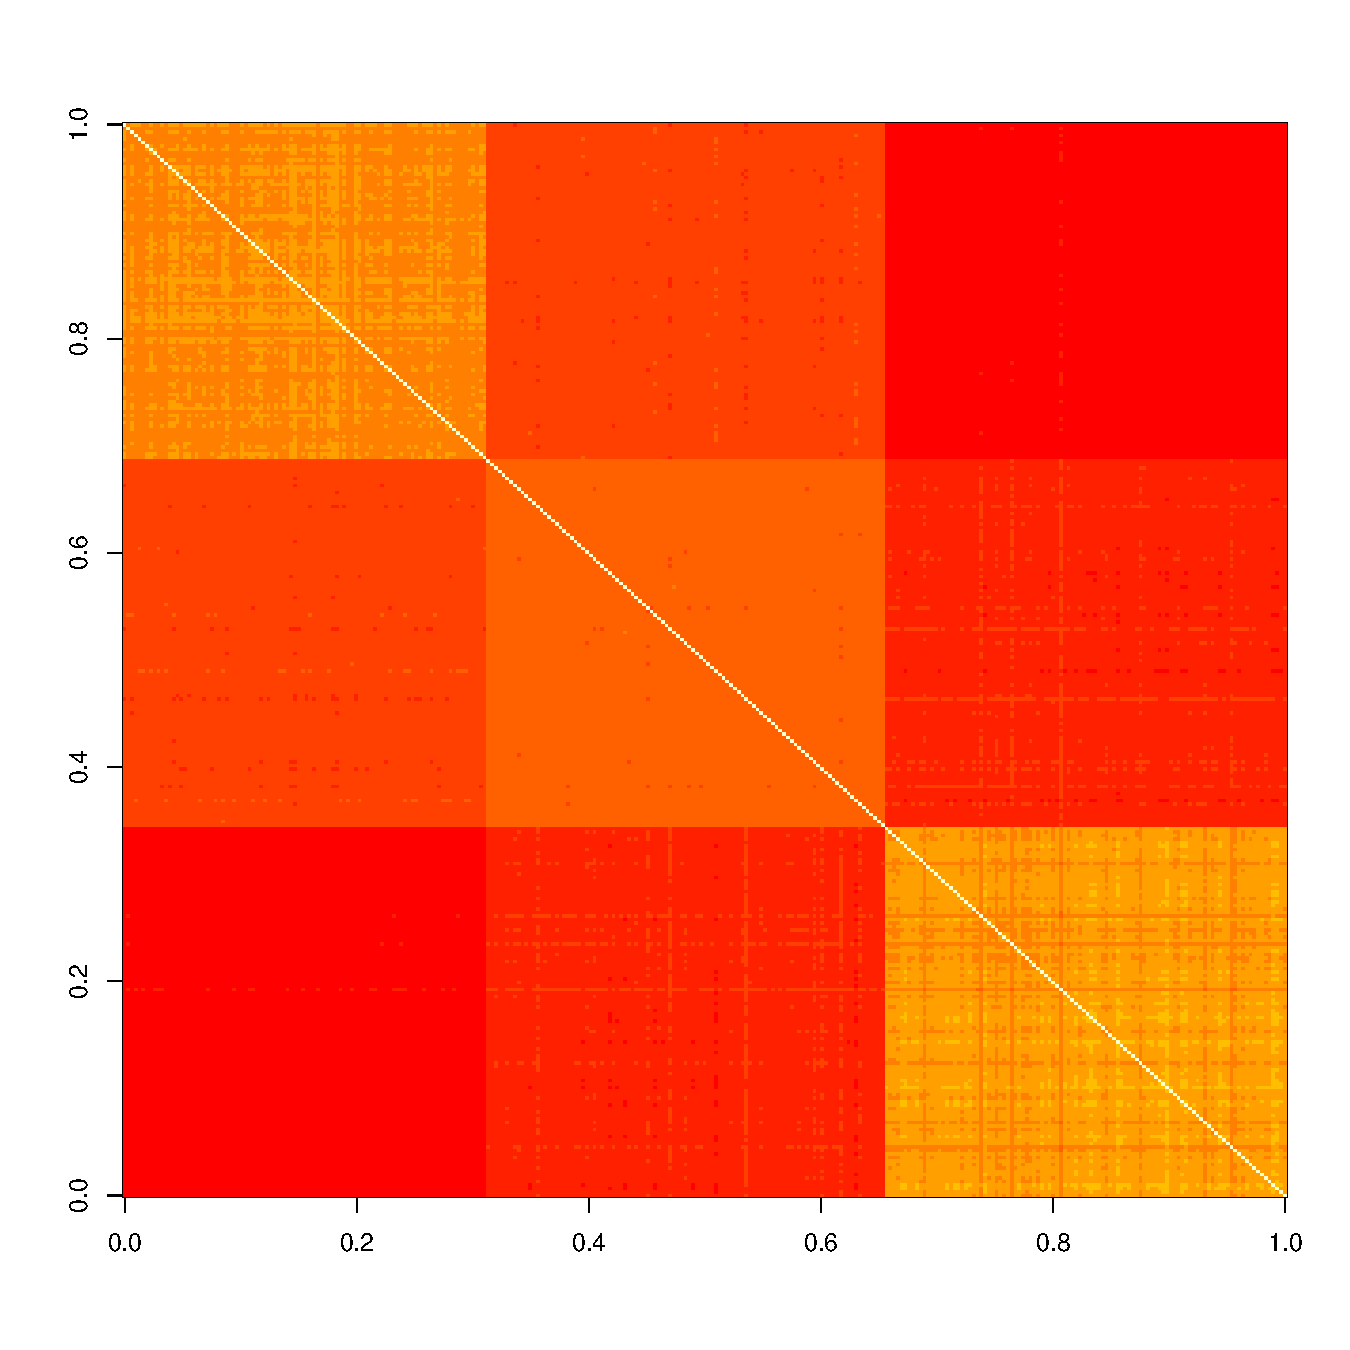
\includegraphics[width = 0.5\linewidth]{plots/hdp_eval.pdf}
        \caption{Estimated Correlation Matrix based on subject cluster assignment. Lighter color indicates stronger correlation.}
        \label{fig:1d}
    \end{subfigure}%    
\end{figure}

\subsection{\textbf{Linear Dynamical System}}
We didn't start on this part yet, although we have done some reading in the Murphy book to gain familiarity.

\subsection{\textbf{Hidden Markov Model}}
We have completed the code for generating data from HMMs. We are about half-way through the Gibbs Sampler for sampling from HMM posterior. The sampler we are using is the same as in the Fox et al paper, where we compute the backward messages and then sample from the forward conditional distributions. Will worked on this.

\section{\textbf{Upcoming Progress}}
The hierarchical dirichlet process sampler has emerged as the most difficult component of the project. Fox et al. glossed over many complicated details for sampling from the full conditionals which we needed to dig out of supplements to other papers. However, Jeremiah has spent a lot of time working through the theory part and we anticipate making faster progress going forward. Sampling from the matrix-normal inverse wishart distribution and the linear dynamical system components are the major remaining pieces. The automatic relevance determination prior does not seem too problematic since it is just a conditionally conjugate prior. We probably will not try the Firefly MCMC approach since our data is low-dimensional.

\newpage
\section{\textbf{Plan and Deadlines}}
Key internal deadlines are listed in parentheses.
\begin{enumerate}
\item (3/21) \\Code and visualize a dirichlet process sampler. Visualize with a simple two-dimensional clustering simulation.
\item (3/28) \\Code and visualize a``sticky'' hierarchical dirichlet process sampler. Visualize via a two-dimensional clusters-within-clusters simulation.
\item (4/4) \\Write a sampler for an ordinary (non-switching) linear dynamical system and test with simulation.
\item (4/11) \\Write a sampler for a simple hidden markov model with a fixed number of modes.
\item (4/18) \\Finish sampler from DP and HMM (Will). Finish sampler for HDP (Jeremiah). Write sampler for generative model of LDS (Will).
\item (4/25) \\Integrate HDP with HMM (Jeremiah). Integrate HMM with LDS (Will).
\item (5/2) \\Combine everything together (HDP-HMM-LDS). Prepare draft of final report.
\end{enumerate}

\newpage

%\newpage
\bibliographystyle{unsrt}
\bibliography{update}

\end{document}